\documentclass[12pt, twocolumn]{article}
\usepackage[a4paper, total={6.5in, 10in}]{geometry}
\usepackage{mathptmx}
\usepackage{amssymb}
\usepackage{amsthm}
\usepackage{amsmath}
\usepackage{mathrsfs} 
\usepackage[normalem]{ulem}
\usepackage{enumerate}
\usepackage{mathtools}
\usepackage{graphicx}
\usepackage{hyperref}
\usepackage{blkarray}
\usepackage{mathtools}
\usepackage{wasysym}
\usepackage{caption}
\captionsetup{width=0.95\linewidth, font=footnotesize}
%\usepackage{wrapfig}
\usepackage[none]{hyphenat}
\tolerance=1
\emergencystretch=\maxdimen
\hyphenpenalty=10000
\hbadness=10000

\usepackage{draftwatermark}
\SetWatermarkLightness{ 0.9}
\SetWatermarkText{DRAFT}
\SetWatermarkScale{ 1}
\usepackage[sorting = none, style=ieee]{biblatex}
\addbibresource{Sources.bib} %Import the bibliography file

\begin{document}

	\title{Longitudinal Study of \\ Green Labs Sustainability Contest's Impact on\\ User Behavior and Energy Savings from\\ VAV Fume Hoods. }
	\author{Ziyu Li, Kathryn Ramirez-Aguilar, Brian Zaharatos, and Shannon Horn}
	\date{\today}
	
\twocolumn[{
  \begin{@twocolumnfalse}
    \maketitle
    \begin{abstract}
\noindent This study investigates the impact of a Green Labs Fume Hood and Door Contest conducted at University Colorado Boulder campus, on laboratory user behavior around variable air volume (VAV) fume hoods, laboratory doors, and the associated energy savings using mathematically robust methods. The contest aimed to reduce average sash height of VAV fume hoods, encourage closure of horizontal sliders, and improve door closure compliance for safety and energy savings. Data on vertical sash height, total horizontal slider gap, and door closure statues were collected longitudinally nine times over a three-week period during the contest, and preliminary data were collected in the two months before for comparison. Results showed significant reduction in vertical sash height ($F(3.3, 148) = 4.62, p_{sash} = 0.003$)), leading to estimated average annual energy savings of 2927 kWh (95\% CI: [1120, 4304] kWh)  and cost savings of \$268.3 (95\% CI: [\$102.7, \$394.5]) per fume hood. For the entire building, the estimated annual savings were 497,700 kWh (95\% CI: [190,500, 731,000] kWh) and \$45,610 (95\% CI: [\$17,460, \$67,060]). This study provides detailed methodology for implementing similar non-resource intensive contests in other institutions and quantifying their impact even without continuous energy monitoring systems. 
    \end{abstract}
  \end{@twocolumnfalse}}
]
	
\clearpage

\section*{Background}\label{Sec:Background}
	A vented fume hood is a large laboratory equipment that is enclosed on all sides except the front. The front of the fume hood commonly has a glass sash that can be moved up or down to allow the user to work with hazardous materials inside. Fume hoods in laboratory environments are crucial for protecting lab user health and safety. They provide an enclosed environment to remove hazardous gases or vapors laboratory users might inhale by constantly drawing air out of its vents. Their front sashes, when closed to appropriate heights, also protect users from explosions inside the fume hood, contain chemical spills, and protect products or experiments from certain outside contaminants. 

\begin{figure}[ht]
	\centering
	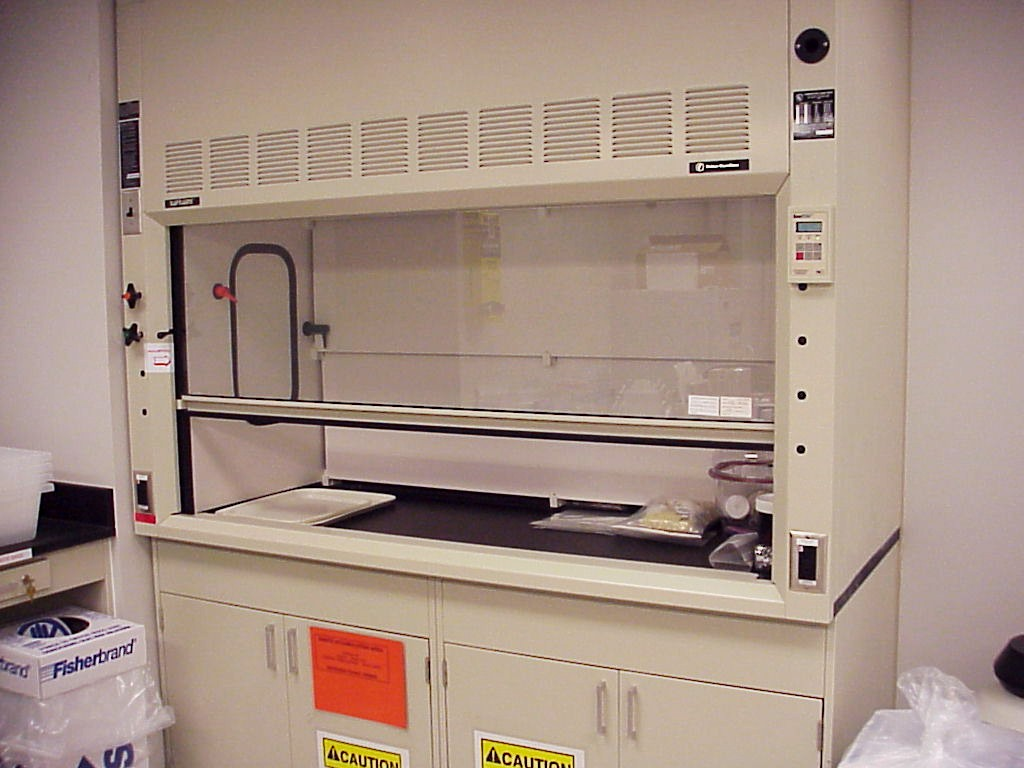
\includegraphics[width=0.9\linewidth]{Images/Other_StandardFumeHood.jpg}
	\caption{A standard vented laboratory fume hood with its vertical sash slightly open. The working height of the fume hood is usually counter height. Users stand in front of the glass sash when using the hood. There are lights inside the hood to illuminate the working space inside the hood. }
	\label{Fig:StandardFumeHood}
\end{figure} 

They are also known to be one of the most energy-intensive equipment in most laboratory buildings -- consuming 40–70\% of the total energy used in modern laboratories with each hood consuming more energy than three homes in an average U.S. climate \cite{Kongoletos2021} , \cite{Mills2005}. The ventilation provided by fume hoods requires high air exchange rates by rejecting conditioned air outwards, which puts a strain on the air conditioning (HVAC) systems in the building \cite{Becerra2018} and requires the HVAC system to use more energy to produce conditioned air to replaced air removed by the fume hoods. 

Constant air volume fume hoods (CAV) are standard in most older laboratories. They pull out a constant amount of air at all times. The newest generation of laboratory fume hoods are variable air volume fume hoods (VAV). They are harder and more expensive to install but draw a variable amount of air based on position of the vertical sash which can lead to potential energy savings with lower sash heights. However, fume hood safety in general, and especially VAV fume hoods energy saving capabilities, are universally not well-known to laboratory users with one study suggesting 49\% to 65\% of the hoods are open over a two-week period in their university laboratories \cite{Park2006}. 

Laboratory sustainability communities have long had the interest of running successful campaigns to educate users and change user behavior around fume hood safety and energy savings. However, recent studies with passive feedback methods have shown lackluster reduction in sash height \cite{Wesolowski2010} and continuous monitoring methods showed significant improvement but can have a costly start-up cost \cite{Kongoletos2021}, making the previous approach unattractive and former straight up unattainable for vast majority of Green Labs programs around the world that lack funding and time resources or have no continuous monitoring technology on their fume hoods. In a university environment, there is also interest from building managers to minimize misuse of fume hoods, as it can impact the ventilation system of the whole building, leading to safety hazards of even non-lab users in a particular building. This is in addition to poor chemical spill containment in an emergency. University facilities management also would like to have concrete analysis on how impactful fume hood sustainability campaigns are in saving energy and cost of operations in VAV fume hoods to inform future decisions when building new laboratory buildings or renovating older ones. With all these interests in mind, CU Green Labs decided to conduct an experiment by running a Fume Hood and Door Contest at University of Colorado Boulder's (CU Boulder) Jennie Smoly Caruthers Biotechnology Building (JSCBB) with its roughly 170 VAV fume hoods. 
	
\begin{figure}[ht]	
	\centering
	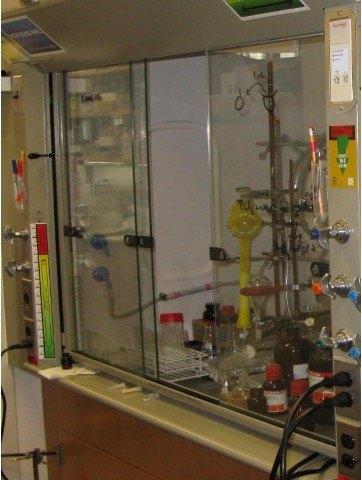
\includegraphics[width=0.4\textwidth]{Images/Other_JSCBBFumeHood.jpg}
	\caption{A standard vented laboratory fume hood in JSCBB with its glass horizontal slider wide open but vertical sash shut. Notice that there are ruler taped on the side, and the green hand sticker are both previous effort by Green Labs which was made standard on campus to remind researchers to shut the vertical sash but no educational materials on correct usage of horizontal sliders. }
	\label{Fig:StandardFumeHoodJSCBB}
\end{figure}

	The CU Green Labs Program has been contributing to fume hood sash management at the CU Boulder campus since the program's inception in 2009. The program has good standing with scientists and other lab personnels on campus through its outreach efforts, presence in other sustainability services such as free mobile back-up freezers, and low cost ultra low temperature freezer space rentals. The program had historically been utilizing its student assistants to run Shut The Sash fume hood sustainability campaigns on a yearly basis, depending on funding and student availability, in other smaller laboratory buildings on campus and wanted to run a Shut The Sash campaign to restart fume hood sash sustainability efforts to rebound from lack of progress during the COVID-19 pandemic. 
	
	In addition to fume hoods, there were ongoing concerns at JSCBB about lab personnels propping laboratory doors open. Leaving laboratory doors ajar would impede the HVAC system's ability to keep a negative pressure in laboratory spaces designed to contain chemical fumes inside a lab in a case of a spill. This could also lead to HVAC system needing more energy to compensate for this unwanted equalization of pressure. Furthermore, the JSCBB building has VAV fume hoods that include horizontal sliders. Many lab personnels are not used to this, as it is not standard. See Figure \ref{Fig:StandardFumeHoodJSCBB}. It is proposed as a way to protect researchers while actively working at a fume hood. The researcher would reach their hands around the glass planes that would be in front of their faces, while working with material inside the hood. There have not been efforts in advocating for correct usage of the horizontal sliders and it has been suspected that the fume hoods provide poor fume capture with vertical sash down but horizontal sliders open. 
	
	With all the interested parties involved, CU Green Labs conducted the 2022 JSCBB Fume Hood and Door Contest during a three week period in the summer of 2022 in partnership with CU-Boulder Facilities Management and Environmental Health \& Safety (EH\&S) with the aims to assess energy savings from its traditional campaign's impact in lowering average sash heights, lowering total horizontal slider gap, and encouraging lab door closures. Through this paper, we hope to provide a road map for conducting similar campaigns in other universities and institutions with minimum hardware needed and examine the role of such campaigns in laboratory sustainability. 

\section*{Methods}\label{Sec:Methods}
Historically, CU Green Lab's fume hood contests were set up so the lab accumulate points when the sash height is 2 inches or below during a three week period. This time frame of three weeks was decided in order to balance between having the contest long enough for users to form a habit of closing the sash when not actively using the fume hood and the stamina and man-hours needed for team members to run the contest. The points accumulated by each lab were each entered as a raffle ticket for the final event where a few labs would be picked for a prize. During the contest, data on sash height, total slider gap, and door closure statues were collected longitudinally for analysis. This section are broken up into several subsections, detailing our approach for setting up the contest, main contest strategies, and the associated materials and resources needed.
\subsection*{Before the Contest}\label{Sec:BeforeContest}
Since the contest involved hundreds of laboratory users and building personnels, we needed permissions from stakeholders -- Campus EH\&S, JSCBB Building Management, and Facilities Management Engineering and Operations -- to ensure safety, access, and ethical standards are met during the campaign.  We then requested funding for three \$100 gift cards for any restaurants of the winning lab's choosing. This price was chosen because this is something the whole lab can enjoy, the idea is that the whole lab group would use this gift card and go out together to a restaurant to celebrate. This encourages collaborative effort of the lab and can potentially increase the chances of discussions around in their labs, in addition to encouraging friendly group competition.

Green Labs made flyers to advertise the contest, picked out tabloid sized fume hood posters to replace old posters in the existing Green Labs poster holders previously placed around the building and heavily revised both materials with stakeholders to ensure accuracy and friendly tone of messaging. From our past experiences, many lab users already knew potential safety issues with leaving the fume hood open when not in use but they still fail to close the fume hood due to habit. We addressed issues of habit using the three week time of the contest, and re-enforced the safety and energy-saving facts some researchers might not know through these posters. The flyers were taped to the same existing poster holders, participating lab doors, and on the walls of community rest areas. A slide-styled version of the flyer was also created for TVs around the building with the help of JSCBB building managers. We paid special attention to participant consent and allowed lab personnels to opt-out of the contest by emailing us any time before the contest started. Amazingly, no labs opted out of the contest and some company owned spaces in the building emailed us to asking to opt-in, even without prizes, into the contest.

Additionally, we collaborated with our EH\&S partners and other facilities managers to acquire a list of fume hoods, their fume hood identification numbers, their corresponding room number and labs that own the fume hoods. This information was compiled and verified on the ground by student assistants to ensure accuracy. During this process, all lab doors were identified and mapped. There were some companies renting laboratory spaces in the building which due to university policy, will not be allowed to receive gift card prizes as part of the contest. Their access was also restricted to student assistants.  These fume hoods and doors were identified and did not officially participate in the contest. 

Next, two preliminary data sets were collected one month apart on all fume hoods and one data set was collected for doors before the contest.  The data collected included the sash height in inches, total horizontal slider gap in inches, and door closure status in "Yes" or "No" binary. This was done so we have a baseline we can compare the results of the contest to. 

\subsection*{Main Contest Strategies}\label{Sec:ContestStrategies}
The contest induced a longitudinal study, where we took measurements (sash height, total slider gap, and door status) repeatedly over a three week period on the same experimental units (each participating fume hood or doors). The treatments of the contest involves multiple campaign strategies.

\subsubsection*{Strategy 1: Contest Scoring Cards}\label{Sec:Strategy1}
The day contest started, scoring cards were attached to every participating fume hood above the glass sliders so it is in the line of sight of the fume hood user but no impeding in their work. Slightly modified context cards were taped to participating lab doors near the handle. Again, these were in the line of sight of the lab door user but not impeding its functions. 

\begin{figure}[ht]	
	\centering
	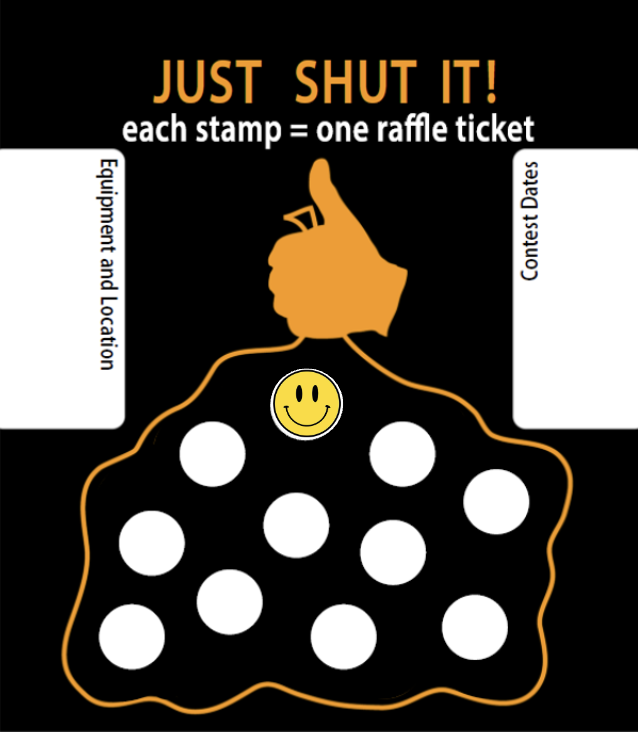
\includegraphics[width=0.31\textwidth]{Images/Contest_JustShutIt.png}
	\caption{A contest card made for the fume hood with one smiley face sticker. We wrote contest dates on the blank space on the right of the card, and fume hood number on the right. The empty circles were possible smiley faces possible for this equipment. }
	\label{Fig:JustShutIt}
\end{figure}

These contest cards acted as score keeping notes for us and physical reminders to laboratory users that the contest was in session. We hoped that seeing these score cards on different fume hoods potentially motivated friendly competition within the same laboratory space, and seeing how many potential raffle tickets the lab could earn motivated group behavior change. We collected these cards at the end of the contest to tally the amount of raffle tickets a lab earned.

\subsubsection*{Strategy 2: Fume Hood Posters}\label{Sec:Strategy2}
As briefly mentioned in \hyperref[Sec:BeforeContest]{Before the Contest}, fume hood themed tabloid sized posters were created and approved by all stakeholders and put up in all existing poster holders in the building. These posters were also rigorously workshopped to ensure good aesthetic and positive tone of messaging. We aimed to educate lab users about energy saving potentials and safety surrounding shutting the fume hood without shaming laboratory users, which could create unnecessary hostility and tension that could impede future sustainability campaigns.  
\begin{figure}[ht]	
	\centering
	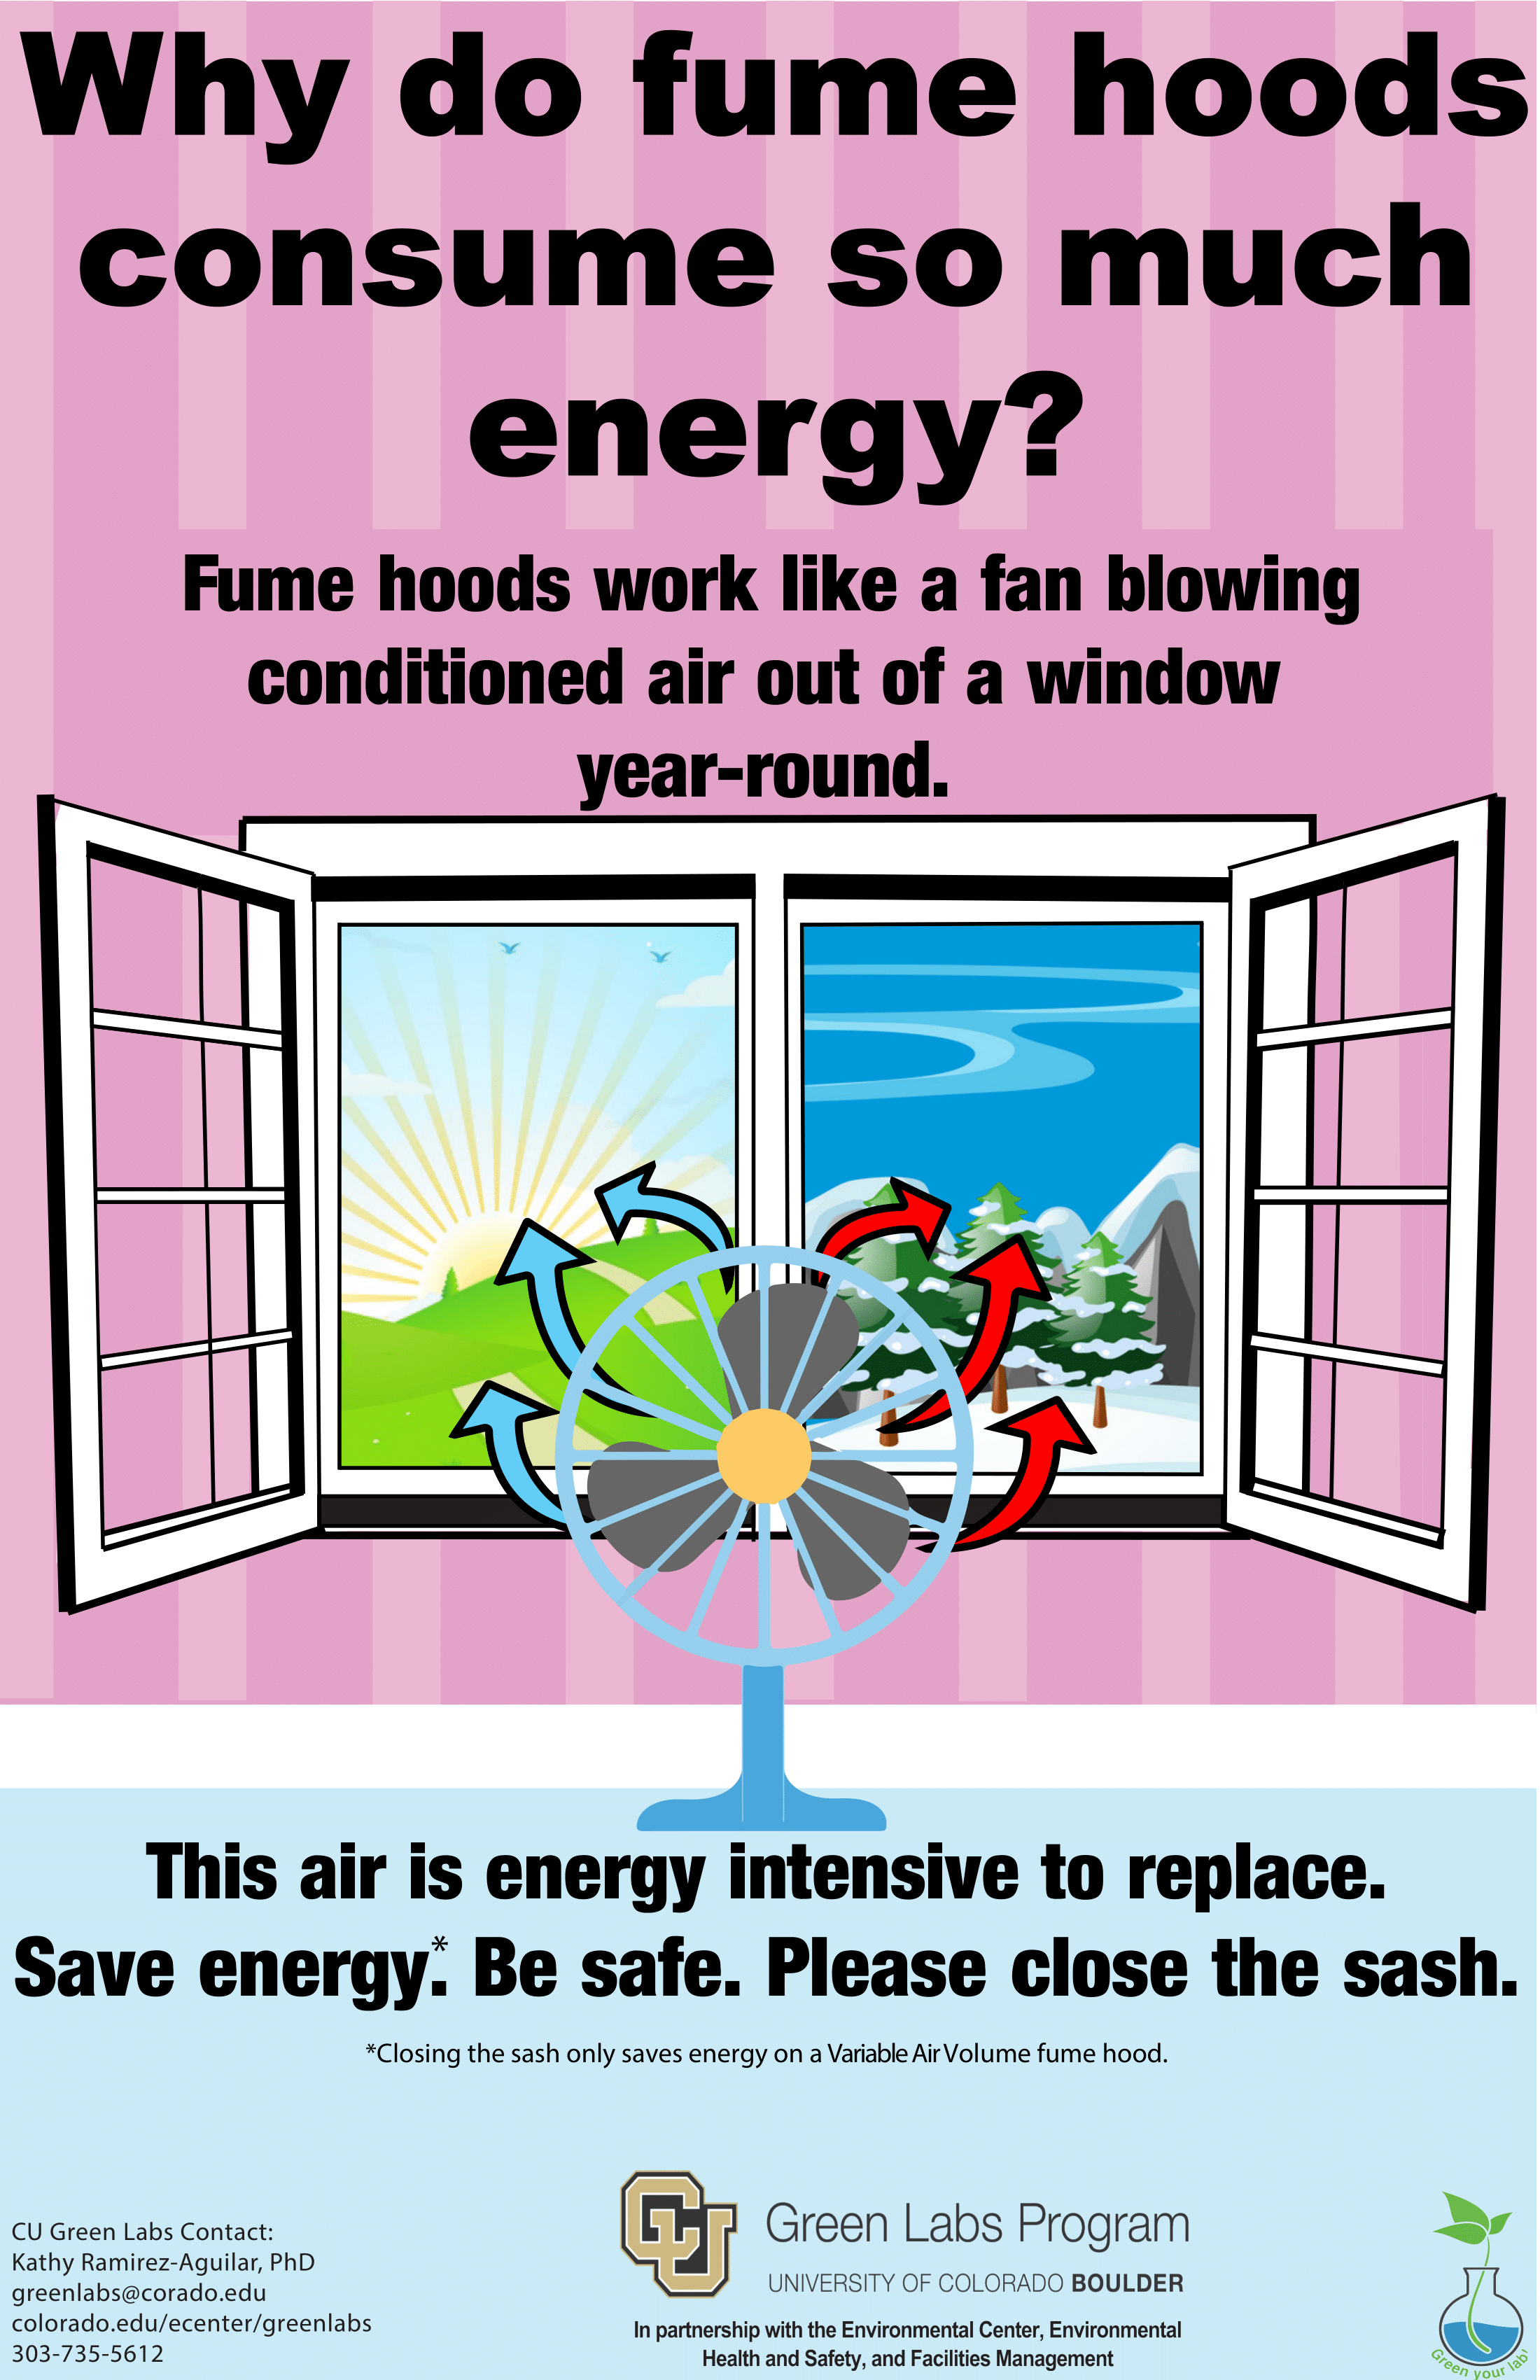
\includegraphics[width=0.4\textwidth]{Images/Contest_FumeHoodFanPoster.png}
	\caption{A representative poster for one out of four posters picked out for the campaign. }
	\label{Fig:FumeHoodFan}
\end{figure}

As shown in Figure \ref{Fig:FumeHoodFan}, a typical fume hood poster had cohesive colors and unique graphics, with titles that were easy to read and straight to the point. There is usually also a message to call for action in a non-offensive way. In this case, it is ''Be safe. Please close the sash." In addition to education value provided by these posters, they also served as a visual reminder about the active contest. 

\subsubsection*{Strategy 3: Lab Visits}\label{Sec:Strategy3}
 Student assistant laboratory visits was the most important part of the contest. Undergraduate student assistants working for CU Green Labs wore laboratory appropriate attires such as long pants, closed toed shoes, goggles, as well as identifying markers such as name tags and a Green Labs badge when visiting the labs. They carried a clipboard with data collection sheets indicating locations of fume hoods and doors to record vertical sash height, total horizontal slider gap, and if the doors were open or closed. All data collected from horizontal sliders and vertical sash were rounded with the tolerance of $\pm 1/4$ inches. Assistants scanned and inputted data in a shared documents after each collection, which often took a pair of assistants 4 hours for the whole building. 

\begin{figure}[ht]	
	\centering
	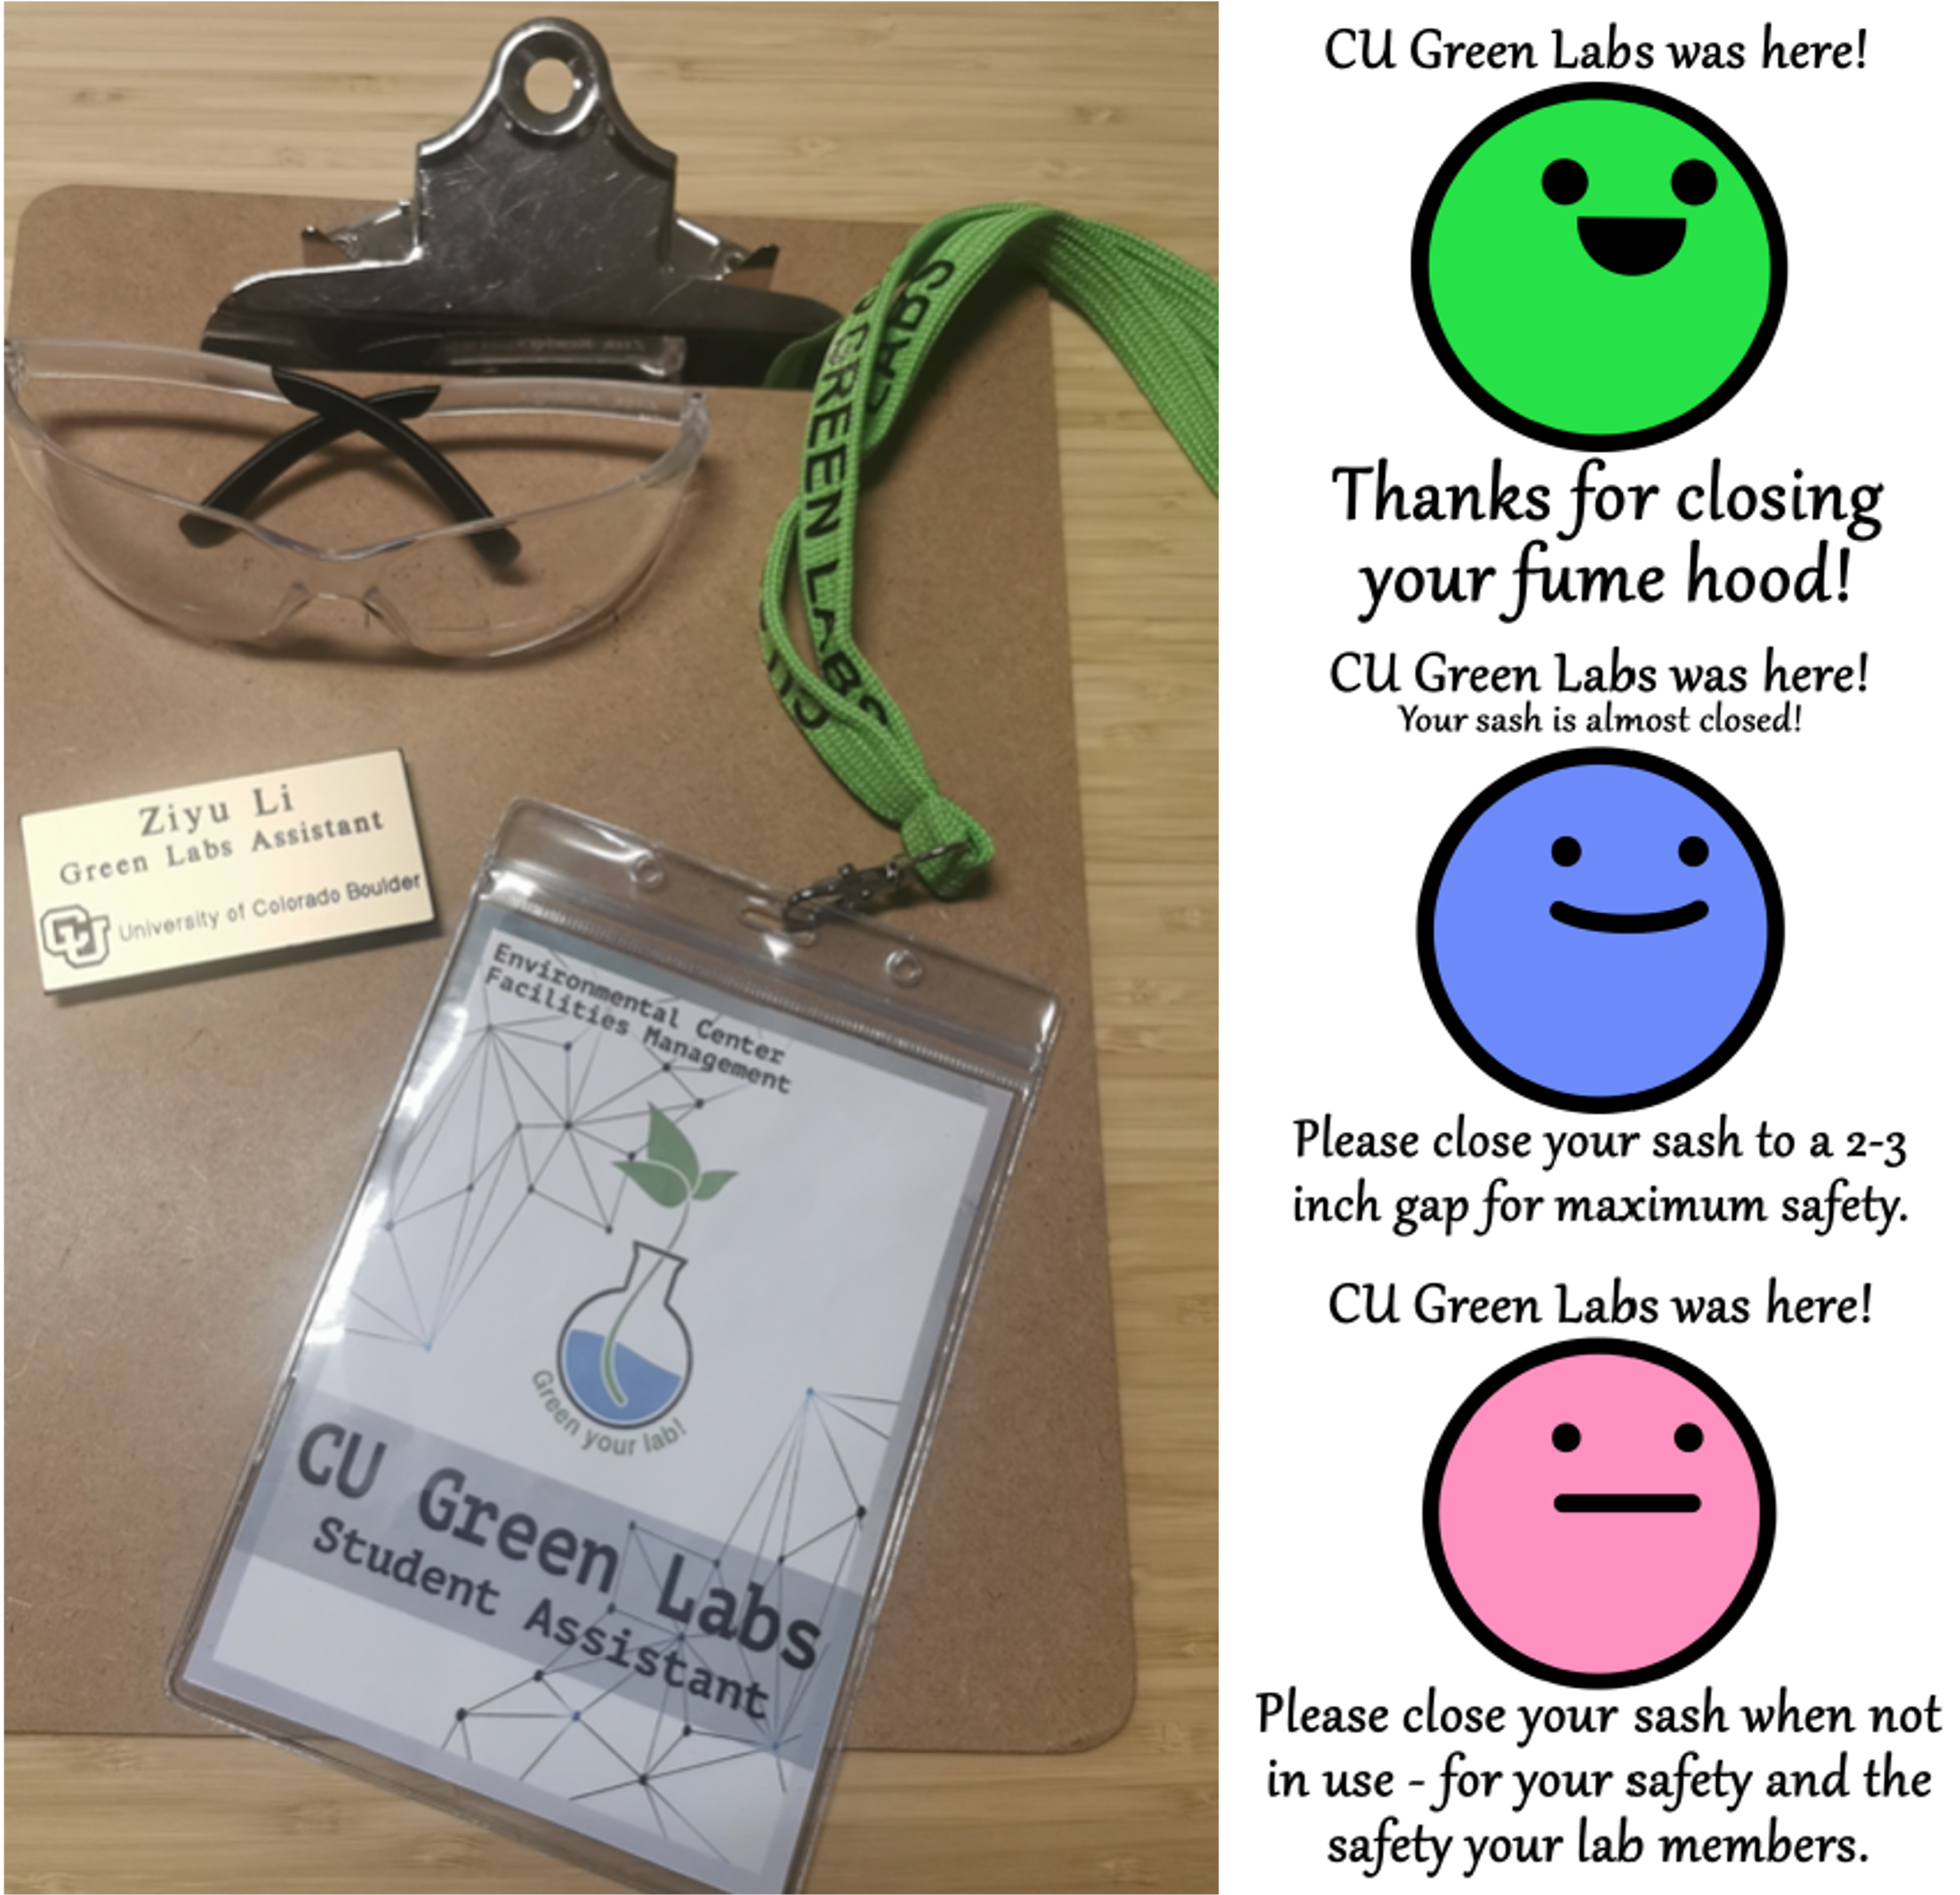
\includegraphics[width=0.45\textwidth]{Images/Contest_ClipboardAndSmiley.png}
	\caption{On the left, image shows a  representative kit for student assistants to bring to laboratory visits. On the right, the figure shows three different smiley face cut outs with messages ranging from positive to slightly negative to encourage better fume hood user behavior with regard to closing the vertical sash. }
	\label{Fig:ClipboardSmiley}
\end{figure}

While collecting data, assistants also left a smiley face note on the fume hood sash to indicate to lab members that the assistants had visited and how well the fume hood did. As shown by Figure \ref{Fig:ClipboardSmiley}, if the vertical sash was 2 inches or under, the fume hood received a green smiley face. If it was14 inches and higher, they received a pink unhappy face. These smiley face notes were placed on the outer layer of the fume hood sash to avoid assistants coming in contact with material inside the fume hood and to maximize visibility. 

While one important purpose of these visits was collecting data for analysis, the main reason for the visits was to remind laboratory users that frequent checks were performed during the duration of the contest. This pressured laboratory users to be more mindful of their behaviors. Sometimes this could backfire when a lab member was unhappy with Green Labs previously before the contest or dislike lab visits in general. We hoped that giving labs a chance to opt-out would mitigate tension between Green Labs and researchers, but any conflicts that arose would have been remedied by the friendly and knowledgeable Green Labs assistants visiting those labs.  We provided training for possible intense interactions that could happen during these visits, and deploy a buddy system where two assistants always stuck together during visits to encourage positive interactions and accurate information delivery. Student assistants were encouraged to chat with lab members to create a friendly atmosphere when visiting. 

\subsubsection*{Strategy 4: Ice Cream Social}\label{Sec:Strategy4}
The assistants on their last data collection trip verbally announced the date and location of the end-of-contest event to lab members. We hang flyers at all participating labs' doors to remind lab users about the ice cream social event where the raffle drawing happened. While this strategy did directly impact the result of the contest when being announced, we hoped it helped us build a community where sustainable behaviors was rewarded and people who have contributed to better safety and sustainability were recognized. This could help us with future Green Lab contests in the building. 

\section*{Analysis}\label{Sec:Analysis}
The contest produced 92 fume hood vertical sash height, 75 total horizontal slider gap, 77 door closure statue usable data units over 9 data collection dates in the duration of the contest. Within those units, both vertical sash height and total horizontal slider gap contained two preliminary data observations and the doors only one preliminary data observation before the contest. Traditionally, the results of sustainability contests were analyzed qualitatively by looking at average trend over time due to technical skill, time, and small sample limitations. We aimed to produce more robust analysis using longitudinal ANOVA to supplement traditional methodologies to provide insights into if the contest had influenced user behaviors in a significant way, and if so when did it take effect. We also analyzed the results post-contest to estimate annual energy and cost savings assuming behavior post-contest was maintained for rest of the year, which we believe was a reasonable assumption with monthly fume hood checks performed by student assistants as behavioral reinforcements after the contest and habit forming due to the length of the contest. 
\begin{figure*}[ht]	
	\centering
	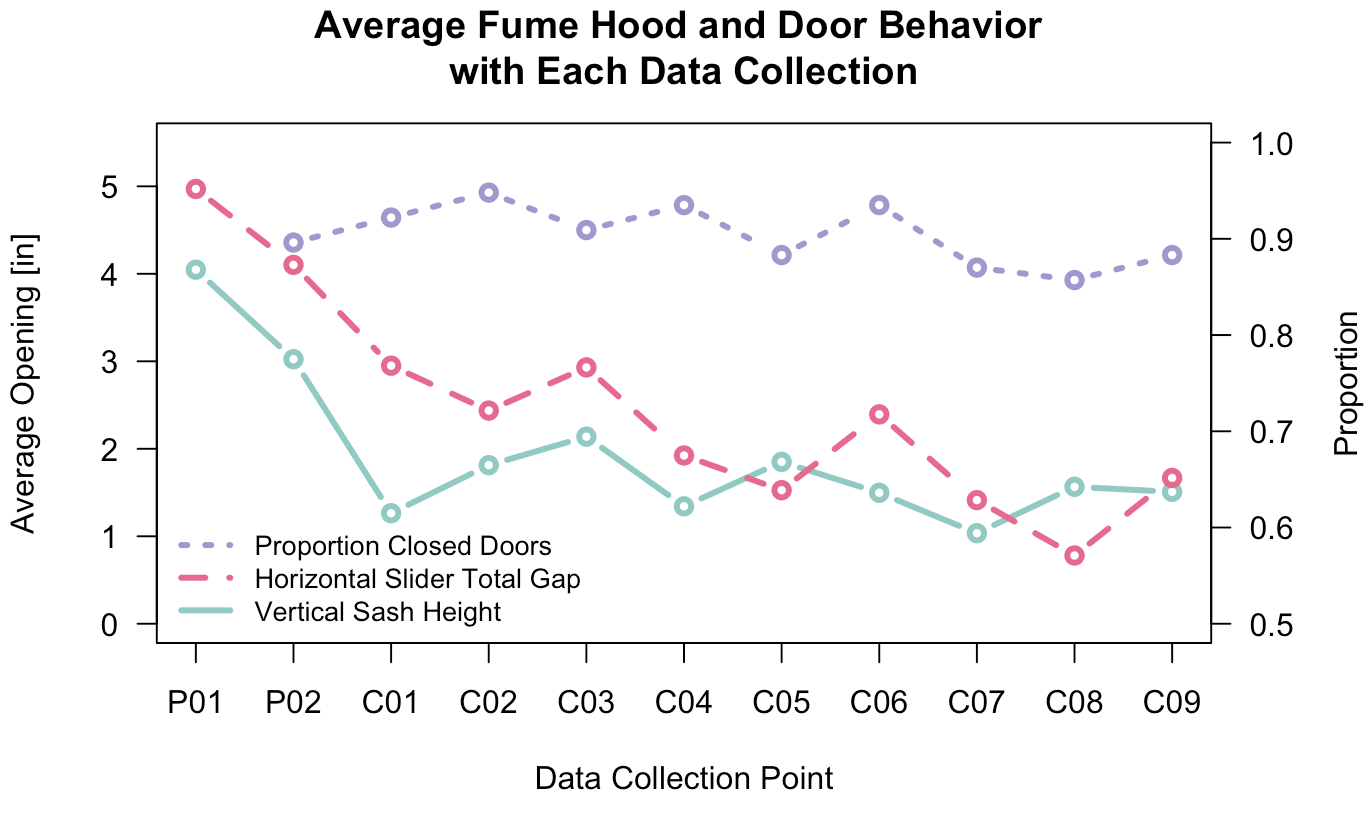
\includegraphics[width=1\textwidth]{Images/FumeHoodAnalysis_AvgTrendAndProportions.png}
	\captionsetup{width=.9\linewidth}
	\caption{The average fume hood vertical sash height, average total horizontal slider gap, and proportion of closed doors with each data collection point. There were two preliminary data collection points, P01 and P02, collected before the contest for vertical sashes and horizontal sliders. There was only one for proportion of closed doors, and it was done at the same time as P02. The rest are from data collected randomly 9 times during the contest. The data collection points are organized chronologically. }
	\label{Fig:AverageTrendsSashSliderDoors}
\end{figure*}

\subsection*{Exploratory Analysis}\label{Sec:ExploratoryAnalysis}
All data collected exhibited strong non-Gaussian behaviors with large spread. Vertical sash height and total horizontal slider gap at every single time point were skewed right, with slider gap slightly less so than sash height. We suspected that was because most fume hood users did use them correctly or used fume hood infrequently enough that they were closed and never touched. This was also true for all the laboratory doors in the building where vast majority of the doors were fully closed. The fume hoods and doors that were fully closed or used correctly often stayed that way throughout the contest. 

From Figure \ref{Fig:AverageTrendsSashSliderDoors}, we observed the average vertical sash height and total horizontal slider gap went down over the duration of the contest. The averages for the second preliminary data collection was lower than the first preliminary data collection, which we expected from previous experiences with similar contests. This was because the act of data collection was also a treatment method as described in  \hyperref[Sec:Strategy3]{Strategy 3: Lab Visits}. For this reason, we only used the first preliminary data as benchmark for comparisons. We did not visually observe significant changes to the proportion of doors closed throughout the contest and therefore hypothesized that the pilot component of the campaign on encouraging door closures did not make an impact on user behavior around doors. For this reason, we did perform further in-depth analysis on proportion of doors closed. 

\subsection*{Longitudinal ANOVA}
Our data involved repeatedly sampled outcome variables -- vertical sash height, total horizontal slider gap, and lab door open status -- which broke the independence assumption that many conventional statistical methods require. Our experiment was a longitudinal study, designed to investigate changes in lab user behavior over time, performing multiple comparisons would decrease the power of the test and increase the chance of misleading or wrong conclusions \cite{SchoberPatrick2018RMDa}. The one-way repeated measure ANOVA, sometimes known as longitudinal ANOVA or within-subjects ANOVA, was a better method for our setting to avoid those issues \cite{StatMethodPsychology} \cite{RComparingGroups}.  We used the \texttt{rstatix} and \texttt{tidyverse} R packages for data manipulation and analysis \cite{rstatix} \cite{tidyverse}. 

First, we performed data cleaning and assumption verification. We removed all fume hood units from the vertical sash height and horizontal slider gap data that were observed to be 0 inches all throughout the contest. We believed that this indicated the fume hood was not being actively used, or the fume hood user(s) already had good habits of closing the sash and sliders fully, and therefore would not show a change in their behavior during the contest. Then, we verified that there were no influential outliers and removed the fume hoods that produced influential outliers if they were present. We defined influential outliers to be 3 standard deviations away from the mean. This left us with 46 fume hood units, each with one vertical sash height observation for each of the eleven data collection slots and 28 fume hood units for horizontal slider gap.   

Then, we examined the normality assumption across each data collection point by performing the Shapiro-Wilk's test. We chose this instead of the traditional Q-Q plot method due to our small sample size. The null hypothesis for the Shapiro-Wilk's test ($H_{0, SW}$) was that normality was met and the alternative hypothesis ($H_{A, SW}$) was that normality was not met. We performed this test across subjects, and discovered extremely small p-values ranging from $p_{\text{sash}, SW} = 1.37 \times 10^{-11}$ to $p_{\text{sash}, SW}  = 1.23 \times 10^{-7}$ for vertical sash height and $p_{\text{slider}, SW} = 4.74 \times 10^{-10}$ to $p_{\text{slider}, SW} =  6.78 \times 10^{-6}$ for horizontal slider gaps which constituted strong evidence for violation of the normality assumption.  This made sense since most fume hoods were being operated correctly. We hoped that despite this violation, the sample means across time would still provide insightful information about the impact of the contest. 

Finally, the sphericity assumption which says variances of the difference between all combinations of related groups must be equal was also possibly violated as variances towards end of the contest were smaller in exploratory data analysis. We used the Greenhouse-Geisser correction method to resolve any issues from sphericity assumption not being met. We constructed the following null and alternative hypotheses for vertical sash and horizontal sliders:
\begin{enumerate}
\item[ ] $H_{0, \text{sash (or slider)}}$: The true means of vertical sash height (or total horizontal slider gap) between each sampling time were the same.
\item[ ] $H_{A, \text{sash (or slider)}}$: At least one of the true means of vertical sash height (or total horizontal slider gap) between each sampling time was different.
\end{enumerate}
In other words, the null hypothesis suggested the contest had no impact on fume hood sash height or slider gap and the alternative hypothesis implied the opposite. The longitudinal ANOVA resulted in the test statistic of $F(3.3, 148) \approx 4.62$ with the corresponding p-value of $p_{\text{sash}} = 0.003$ for vertical sash height and $F(2.96, 80) \approx 1.42$ with the corresponding p-value of $p_{\text{slider}} = 0.243$ for total horizontal slider gap. Hence, we did have extremely strong evidence to suggest that the contest did impact user behavior around the vertical sash but not enough evidence that it had an impact for the horizontal sliders. This made sense as many lab users previously expressed that they had never seen horizontal sliders in their previous institutions and did not know how to use them properly. 

\subsection*{Post-Hoc Analysis}\label{Sec:PostHoc}
In addition to examining the effectiveness of the contest overall, we performed a post-hoc analysis to gain more insights on the data using pairwise t-tests with p-value adjustments. In particular, we were interested in exactly when in the sample collection point did the contest produced the most amount of change in sash height and slider gap. P-value adjustments in the pairwise t-tests were done using the Benjamini \& Hochberg procedure \cite{BH}. This was chosen to not be overly punishing on the number of time-steps being compared.

\begin{figure*}[ht]	
	\centering
	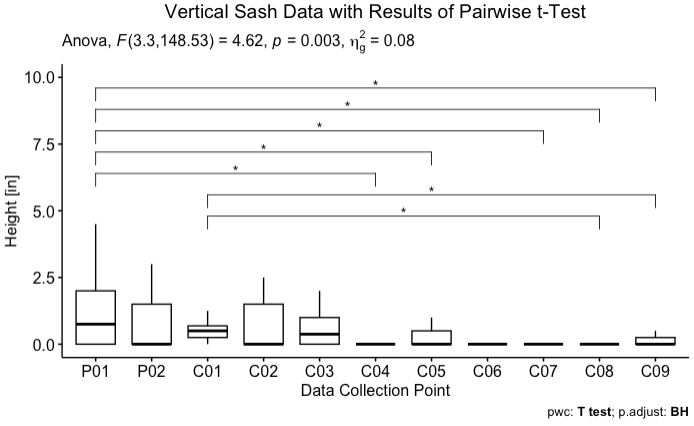
\includegraphics[width=0.95\textwidth]{Images/FumeHoodAnalysis_PairwiseTTestSash.png}
	\captionsetup{width=.9\linewidth}
	\caption{Box plot of vertical sash height for each data collection point with lines indicating statistically significant collection points at the significance level of $\alpha = 0.05$. }
	\label{Fig:PairwsieTTestSash}
\end{figure*}
Figure \ref{Fig:PairwsieTTestSash} shows the first preliminary data set for vertical sash height was significantly different from the fourth, fifth, seventh, eighth and ninth collected during the contest at the significance level of $\alpha = 0.05$. The second data set collected during the contest was significantly different from the eighth and ninth at the same $\alpha$ level. The other pairwise tests not shown were not statistically significant. We also did not find any statistical significantly different pairs for horizontal slider gap which was to be expected as previously through longitudinal ANOVA, we did not find evidence that the contest had an impact on the gaps. 

\subsection*{Energy and Cost Analysis}\label{Sec:Energy}
Energy savings could only be directly assessed via vertical sash height changes as the impact of closed laboratory doors is not well studied, and the impact of horizontal sliders gap on savings is, if any, unknown. There were no continuous energy monitoring systems on each of the fume hoods in the building, we could only estimate true energy savings as the result of lower sash height. Vast majority of fume hood's energy consumption were through the building's HVAC system replacing displaced conditioned air. To quantify this, we needed to first estimate the volumetric flow rate of the fume hoods before and at then end of the contest using the flow rate equation for VAV fume hoods:
\begin{equation}\label{Eq:Flowrate}
V(h) = v_F \cdot w \cdot h
\end{equation}
\newline
Where $V(h)$ is the volumetric flow rate [cfm] of the VAV fume hood which varies approximately linearly with vertical sash height; $w$ is the width [ft] of the fume hood, which is fixed at 6 ft and the same for every fume hood in the building; and $h$ is the height [ft] of the fume hood sash; and $v_F$ is the face velocity [ft/min] of the fume hood and also varies with vertical sash height. We know that, by design for safety, the volumetric flow rate of the fume hood was 100 cfm when the vertical sash was 2 inches or below. And, we calculated the average face velocity of fume hoods in the building at the sash height of 14 inches to be 91 ft/min from experimental data for every single fume hood in the building during installation from EH\&S.  We believed that the average of the experimental face velocity measurements is representative of the \textit{average} fume hood in the building as the data was approximately normal. From this, we calculated the volumetric flow rate of the fume hood to be approximately 636 cfm when the sash was open to 14 inches. Now, we found flow rate at any new sash height observations $h_{new}$ between 2 and 14 inches via interpolation:
\begin{equation}\label{Eq:NewFaceVelocities}
V(h_\text{new}) \approx 100 + (h_\text{new} - 2)\frac{(636 - 100)}{(14 - 2)}
\end{equation}
where $h_{\text{new}}$ is the new sash height in inches. 

Then for vertical sash height, we considered only the first data collection (P01) as vertical sash height observations before the contest and the last (C09) as observations at the end of the contest. We performed bootstrapping by resampling each data of the same size with replacement 2000 times, calculating the mean for each resample. This method enabled accurate estimation of confidence intervals without restrictions on normality of the original data.
\begin{figure}[ht!]	
	\centering
	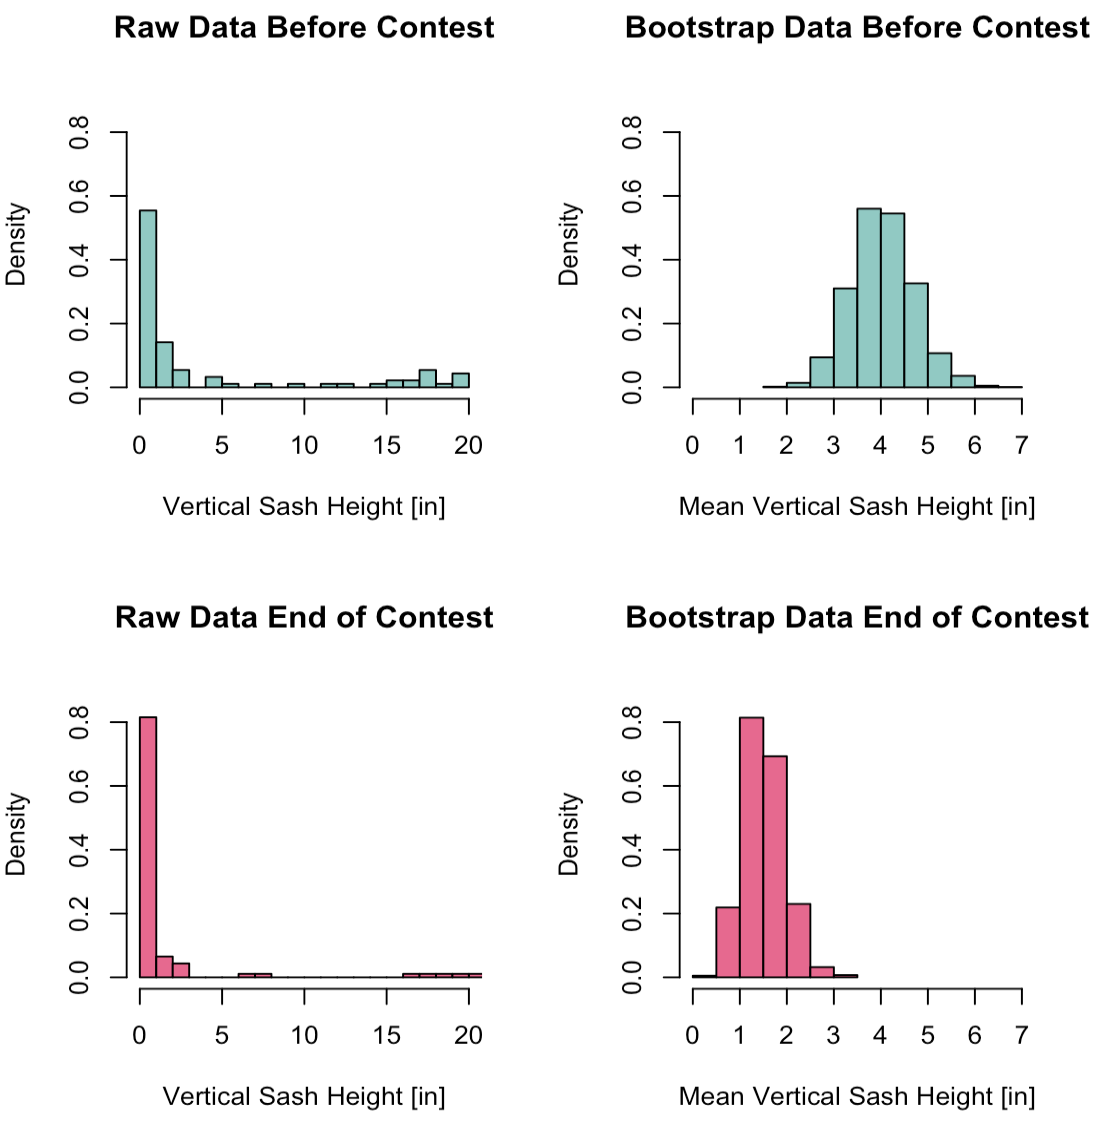
\includegraphics[width=0.48\textwidth]{Images/FumeHoodAnalysis_BootStrapDistribution.png}
	\caption{Top plots show the vertical sash height data distribution before the contest on the left and the bootstrap distribution for the mean of that data on the right. The bottom plots are the same but for data collected at the end of the contest. }
	\label{Fig:BootStrapDistribution}
\end{figure}
\newline
As displayed in Figure \ref{Fig:BootStrapDistribution}, our data were severely skewed and non-normal but the bootstrap distributions of the means were roughly normally distributed with their centers of 4.03 inches before the contest and 1.51 inches at the end of the contest.  We used these bootstrap means to estimate the 95\% empirical confidence interval for the true vertical sash height means to be [2.78,  5.42] inches before the contest and [0.74, 2.43] inches at the end of the contest. Using the interpolation formula provided by Equation \ref{Eq:NewFaceVelocities}, we found the mean volumetric flow rate for each fume hood to be 191 cfm and 100 cfm for before the contest and at the end of the contest. The corresponding 95\% confidence intervals for the average flow rates were [135, 253] and [100, 119] cfm. 

Power from heating and cooling displaced air can be calculated using
\begin{equation}\label{Eq:PowerHeatingCooling}
\begin{aligned}
	P_{\text{heating}} &= 0.89 V \cdot \Delta T_{\text{heating}} \\
	P_{\text{cooling}} &= 0.89 V \cdot \Delta T_{\text{cooling}}
\end{aligned}
\end{equation}
where $P_{\text{heating}}$ and $P_{\text{cooling}}$ were measures of power, in BTUH, that are needed to heat and cool displaced volumetric flow rate of air $V$ measured in cfm; and $\Delta T_{\text{heating}} = 17$, $\Delta T_{\text{cooling}} = 23$ \textcolor{red}{(Citation \& Units? Fact check this!)} were constants for this specific building. Assume that the vertical sash behavior observed lasted the whole year, we multiplied the powers by their corresponding degree heating and cooling days. Degree heating and cooling days were 5125 and 1586 respectively for Colorado in 2022 \cite{CoolingHeating2024}. And the energy used for heating and cooling for the whole year can be re-written as
\begin{equation}\label{Eq:EnergyHeatingCooling}
\begin{aligned}
	E_{\text{heating}} &= P_{\text{heating}} \cdot 5125\\ &= 0.89 V \cdot 17 \cdot 5125\\
	E_{\text{cooling}} &= P_{\text{cooling}} \cdot 1586\\ &= 0.89 V \cdot 23 \cdot 1586
\end{aligned}
\end{equation}
where $E_{\text{heating}}$ and $E_{\text{cooling}}$ were the energy needed to heat and cool the displaced air for the year, measured in BTU. Altogether, these make up the mean total energy the HVAC system had to input for each fume hood and they were 6151 kWh per fume hood, per year before the contest, and 3224 kWh at the end of the contest. And the corresponding 95\% confidence intervals were [4344, 8155] kWh before the contest and [3224, 3851] kWh at the end of the contest. This resulted in a mean of 2927 kWh per fume hood, per year of energy savings with the 95\% confidence interval of [1120, 4304] kWh. 

The complexity of calculating cost associated with HVAC energy savings can vary depending on building design, the institution's heating and cooling energy sources, and cost for energy. For our case, the university used electricity for cooling and steam for heating. The cost of electricity was \$0.1234/kWh and the cost of steam was \$27.418/Klb for 2022 \cite{EnergyCost}. There are 1,194 BTU in one pound of steam \cite{ThermalConversion}, so we calculated that the cost of steam for heating to be \$0.0784/kWh. We calculated the altogether average HVAC cost savings to be \$268.3 per fume hood, per year with the 95\% confidence interval [\$102.7, \$394.5]. 

We scaled our calculations up for the 170 fume hoods in the building and found the average total yearly energy saving to be 497,700 kWh with the 95\% confidence interval [190,500, 731,700] kWh and the average yearly cost savings to be \$45,610 with the 95\% confidence interval of [\$17,460, \$67,060]. The summary of more key calculations and results are in the \hyperref[Sec:Appendix]{Appendix}.

\section*{Discussion}\label{Sec:Discussion}
The contest resulted in a roughly 62.5\% reduction in average fume hood vertical sash height and 47.6\% energy reduction per fume hood per year. Our results were similar to a study from MIT where fume hood monitoring devices have decreased their sash height by an average of 76 \% \cite{Kongoletos2021} but our values were slightly lower due lower before-contest average sash height, compared to that of MIT's, as a result of years of effort for outreach in the community prior to the contest. Our results were significantly better than other methods involving monthly feedbacks \cite{Wesolowski2010} and previous studies on the impact of fume hood contests \cite{Sawyer2019}. We believe our calculated savings as the direct results of lowered sashes were gross under estimates as the method for energy and cost calculations were simple approximates on HVAC energy savings,  not accounting for other ways sash heights impact energy consumption as we did not have real-time energy monitoring for fume hoods like many previous studies did.

The seemingly large confidence intervals for energy and cost savings for the whole building was mostly due to scaling from energy savings from 1 fume hood to 170 fume hoods in the building. Other sources of uncertainty are in the treatment process. Student assistants carried multitude of items that impacted their speed and movement, often times resulted in them not putting the smiley signages up on the fume hood sashes as shown in Figure \ref{Fig:ClipboardSmiley}, which might have diminished contest effectiveness on lowering fume hood sash heights and therefore energy consumption. Although longitudinal ANOVA suggested extremely strong evidence that contest was effective at lowering vertical sash height, and post hoc analysis indicated effects showing starting in the second week of the contest, normality issues with the original data might have impacted the results slightly. Future studies using similar data sets could consider bootstrap sampling for the mean of vertical sash height for each time point, and perform longitudinal ANOVA on the bootstrap samples. However, issues with normality did not impact energy and cost savings calculations. 

Although exploratory data analysis indicated possible downward trend in total horizontal slider gap, there were no statistically significant relationships discovered that could indicate the contest had impacts on horizontal slider gaps. We hypothesized that, as building managers suspected, the lab users might not be aware of correct usage of the horizontal sliders. While they did not impact energy consumption, in the way that we quantified energy consumption by a fume hood, larger gaps could cause ventilation concerns in laboratories and the whole building. CU Green Labs also had significantly less signages, posters, and other educational material on horizontal sliders due to funding and time constraints. This result had influenced the university's decision to not install fume hoods with horizontal sliders in new lab buildings. 

There were no observed changes in door closure rates. This also made sense as throughout the contest, student assistants found that many of these doors were open because they were broken and unable to be physically closed or locks were malfunctioning. Many of these doors were fixed and were able to be closed as a direct result of the contest, but scheduling maintenance took longer than the time period during the contest where progress was measured. This may have resulted in unmeasured energy savings. 

Other unmeasured and unmeasurable benefits of the contest included better ventilation due to closed sashes which could lead to better health, better pressure management between laboratory for lower chances of contamination spread in cases of emergency, increased awareness of safety and sustainability involving fume hoods and laboratory doors which can result in more receptiveness in future Green Labs initiatives. 

\section*{Conclusion}
The CU Green Lab's 2022 JSCBB Fume Hood and Doors Contest caused statistically significant ($F(3.3, 148) = 4.62, p_{sash} = 0.003$) decrease in average vertical sash height with significant changes observed starting at beginning of second week (adjusted $p_{P01,C04} = 0.041$). The contest resulted in estimated average HVAC energy savings of 2927 kWh (95\% CI: [1120, 4304]) and the associated cost savings of \$268.3 (95\% CI: [\$ 102.7, \$394.5]) per fume hood per year. For the whole building of roughly 170 fume hoods, the contest saved an average of 497,700 kWh (95\% CI: [190,500, 731,000] kWh) HVAC energy savings and \$45,610 (95\% CI: [\$17,460, \$67,060]) of energy cost savings per year. Both were underestimates. There were no statistically significant impact on fume hood horizontal slider gaps and door closure rates due to suspected lack of previous education, adequate contest targeted treatment and timely maintenance. 

The results were almost as good as automatic monitoring and alarming systems on fume hoods, which could be costly, but definitely better than previous studies involving Green Labs initiatives such as monthly feedbacks and contests. Our study offers promising prospects for institutions with new or low-funding Green Labs programs aiming to save fume hood energy. It provides detailed roadmap for contest materials and procedures, along with a simple yet thorough method for quantifying energy savings in the absence of real-time energy monitoring systems. By demonstrating the effectiveness of fume hood contests using transparent and mathematically robust methods, this study contributes the growing body of evidence supporting the importance of sustainability initiatives in laboratory institutions for saving energy, improving safety, and saving operational cost. 
\onecolumn
\section*{Appendix}\label{Sec:Appendix}
\begin{table*}[h]
\centering
\captionsetup{font=normalsize, width = 0.8\textwidth}
\caption{Cost and Energy Calculation Summary}
\begin{tabular}{c|c|c}
\textbf{} &\textbf{Mean} & \textbf{95\% Confidence Interval} \\ \hline \hline
\begin{tabular}[c]{@{}c@{}} Vertical Sash Height [in]\\ (Before Contest; End of Contest)  \end{tabular}	& 4.03; 1.51	& [2.78, 5.42]; [0.74, 2.43]	\\ \hline
\begin{tabular}[c]{@{}c@{}}Volumetric Flow Rate [cfm]\\ per Fume Hood \\ (Before; End) \end{tabular}	& 191; 100	& [135, 253]; [100, 119]\\ \hline
\begin{tabular}[c]{@{}c@{}}Power for Heating [BTUH]\\ per Fume Hood \\ (Before; End) \end{tabular}          &2887; 1513	& [2039, 3827]; [1513, 1807] \\ \hline
\begin{tabular}[c]{@{}c@{}}Power for Cooling [BTUH]\\ per Fume Hood \\ (Before; End)  \end{tabular}          &3906; 2047	& [2758, 5178]; [2047, 2445] \\ \hline
\begin{tabular}[c]{@{}c@{}}Energy for Heating [$10^6$ BTU]\\ per Fume Hood, per Year \\ (Before; End) \end{tabular}          &14.8; 7.75	& [10.4, 19.6]; [7.75, 9.26] \\ \hline
\begin{tabular}[c]{@{}c@{}}Energy for Cooling [$10^6$ BTU]\\ per Fume Hood, per Year \\ (Before; End) \end{tabular}          &6.19; 3.25	& [4.37, 8.21]; [3.25, 3.88] \\ \hline
\begin{tabular}[c]{@{}c@{}}Total Energy [kWh]\\ per Fume Hood, per Year \\ (Before; End) \end{tabular}          &6151; 3224		& [4344, 8155]; [3224, 3851] \\ \hline
\begin{tabular}[c]{@{}c@{}}Savings for Heating\\ per Fume Hood, per Year \\ (Energy [kWh]; Cost [\$]) \end{tabular}          &2063; 161.68	&[790, 3034]; [61.88, 237.73] \\ \hline
\begin{tabular}[c]{@{}c@{}}Savings for Cooling\\ per Fume Hood, per Year \\ (Energy [kWh], Cost [\$])\end{tabular}          &864; 106.61		&[331, 1270]; [40.80, 156.76] \\ \hline
\begin{tabular}[c]{@{}c@{}}Total Savings\\ per Fume Hood, per Year \\ (Energy [kWh], Cost [\$])\end{tabular}          &2927; 268.3		&[1120, 4304]; [102.7, 394.5] \\ \hline \hline
\begin{tabular}[c]{@{}c@{}}Building Energy Savings [kWh]\\ per Year\end{tabular}	&497,700               & [190,500, 731,700]                                                                                    \\   \hline
\begin{tabular}[c]{@{}c@{}}Building Cost Savings \\ per Year\end{tabular}	& \$45,610             & [\$17,460, \$67,060]                                                                                    \\ 
\end{tabular}
\label{Tab:Summary}
\end{table*}

\clearpage
\printbibliography
	

\end{document}